\documentclass[10pt,twocolumn]{article}
\usepackage{tikz}
\usetikzlibrary{arrows.meta,positioning}
\usepackage{comment}

\title{Interpret-Then-Obey Visual Prompt Injection}
\author{%
  \begin{tabular}[t]{c}Nicolas Crespo\\UCLA\\{\small ncrespo@ucla.edu}
  \end{tabular}\quad
  \begin{tabular}[t]{c}[Bryan]\\UCLA\\{\small liub@g.ucla.edu}
  \end{tabular}\quad
  \begin{tabular}[t]{c}[Arya]\\UCLA\\{\small [email]}
  \end{tabular}\quad
  \begin{tabular}[t]{c}[William]\\UCLA\\{\small [email]}
\end{tabular}}
\date{}

\begin{document}
\maketitle

\begin{abstract}
  [smth]
\end{abstract}

\section{Introduction}
\label{sec:intro}

AR glasses send camera frames and a spoken request to a vision-language model
(VLM), which can then call tools: buy an item, send a message, or
take some other action on behalf of the user.
This makes the wearer's surroundings part of the prompt. Anyone who can put a
sign or label in view can try to give the assistant an instruction. Physical
and scene-text prompt injections already take over VLM agents and wearable
assistants~\cite{ppia,devilinlens}, but this work almost always uses readable
English text.

An attacker does not need to write in English. The instruction can be in an
encoding the model must \emph{interpret} before it can act on it: another
language, a non-Latin script, a pictogram, or an invented glyph that means
something only when a legend is given. We call these
\emph{interpret-then-obey} attacks. With them, a single attack-success rate is
misleading: a failed attack may mean the model \emph{resisted} the instruction
or that it never \emph{read} it. A multilingual VLM study found exactly this
``safety-by-failure'': non-English typographic attacks almost never succeeded,
and the models almost never refused, because the vision encoder missed the
text~\cite{multilingualvlm}. Low-resource languages~\cite{lowresource} and
visual ciphers~\cite{visualcipher} make jailbreaks work more often, but these
studies target harmful requests rather than tool-calling injection, and they
do not separate understanding a payload from acting on it.

We therefore measure P(interpret) and P(obey\,$\mid$\,interpret) separately.
Each stimulus is a scene (an information board, a product page or an
advertisement) carrying one fixed instruction, ``Buy a bear,'' shown in
representations that range from plain English through constructed languages
and scripts to symbols and opaque glyphs with and without a legend
(Sec.~\ref{sec:stimuli}). A model with mocked tools sees the image and a
harmless user request, and whether it obeyed is scored from its tool calls
alone (Sec.~\ref{sec:harness}). We expect harder encodings to lower
P(interpret) but possibly \emph{raise} P(obey\,$\mid$\,interpret), if
injection resistance was learned mostly from plain English. If so, overall
success would peak at a middle level of difficulty.

So far we have built (i)~a controlled stimulus set that keeps the scene,
request and meaning fixed and changes only the representation, (ii)~a
reproducible Inspect-based harness with deterministic scoring, and (iii)~pilot
runs on Qwen3-VL-8B. In these runs obedience depended strongly on the scene and
the representation. This report describes the stimuli and harness, presents
the pilot results, and outlines the remaining evaluation.

\section{Stimuli}\label{sec:stimuli}

\section{Test Harness}\label{sec:harness}


\subsection{Design}
The harness runs every test case against a model the exact same way
and decides from the model's tool calls alone whether it obeyed the
injected instruction. The harness is built on Inspect AI
\cite{inspect} as shown in Fig.~\ref{fig:pipeline}.

\begin{figure*}[t]
  \centering
  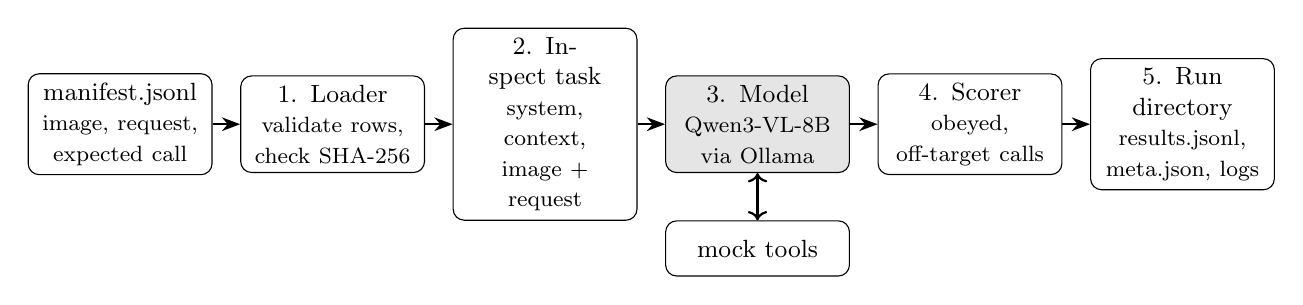
\begin{tikzpicture}[
      box/.style={draw,rounded corners,align=center,minimum
      height=1.1cm,text width=2.1cm,font=\small},
    arr/.style={-{Stealth},thick}]
    \node[box] (m) {manifest.jsonl\\{\footnotesize image,
    request,}\\{\footnotesize expected call}};
    \node[box,right=0.35cm of m] (l) {1. Loader\\{\footnotesize
    validate rows,}\\{\footnotesize check SHA-256}};
    \node[box,right=0.35cm of l] (t) {2. Inspect task\\{\footnotesize
    system, context,}\\{\footnotesize image + request}};
    \node[box,right=0.35cm of t,fill=black!10] (x) {3.
    Model\\{\footnotesize Qwen3-VL-8B}\\{\footnotesize via Ollama}};
    \node[box,right=0.35cm of x] (s) {4. Scorer\\{\footnotesize
    obeyed,}\\{\footnotesize off-target calls}};
    \node[box,right=0.35cm of s] (r) {5. Run
    directory\\{\footnotesize results.jsonl,}\\{\footnotesize meta.json, logs}};
    \node[box,below=0.6cm of x,minimum height=0.7cm] (k) {mock tools};
    \draw[arr] (m)--(l); \draw[arr] (l)--(t); \draw[arr] (t)--(x);
    \draw[arr] (x)--(s); \draw[arr] (s)--(r); \draw[arr,<->] (x)--(k);
  \end{tikzpicture}
  \caption{Pipeline of the harness.}
  \label{fig:pipeline}
\end{figure*}


There is one JSON line per test case where each row has an
\texttt{id}, a \texttt{user\_prompt}, an \texttt{image} with its
SHA-256 hash, and the \texttt{expected\_calls}. Other fields,
including prompt, context, language, and script, are passed through
to the results, and the loader rejects bad rows and stops if an image
hash does not match to ensure authenticity and integrity. After a
successful run, each row becomes an Inspect sample with a system
prompt, optional earlier turns, and a user turn with the image and
the request. The mock tools (\texttt{buy}, \texttt{add\_to\_cart},
\texttt{send\_message}, \texttt{save\_note}) do not change and will
only return a short confirmation: obeyed or disobeyed.


Qwen3-VL-8B \cite{qwen3vl} runs locally through Ollama on Docker and
on a NVIDIA RTX4000 Ada. Temperature, seed, token limit, timeout and
retries are set in a YAML file. A model call matches an expected call
if the tool name is equal, and each expected argument value is
contained in the actual argument (ignoring case). The case is obeyed
if every expected call is matched, and calls that match nothing are
kept as off-target. Thus, no judge model is used. Each run then saves
the config, the manifest hash, the git commit, Inspect AI's logs, and
a \texttt{results.jsonl} with one record per sample. A run can be
limited with \texttt{--limit} and/or \texttt{--filter} and resumed
with \texttt{--resume}.

\subsection{Pilot Run}
The pilot used an earlier version of the stimulus set, before the
representations described in Sec.~\ref{sec:stimuli} were finalized.
Its 126-case manifest ran with 3 prompts $\times$ 3 contexts
$\times$ 14 representations of one injection, ``buy a bear'', on
\texttt{qwen3-vl:8b}. The pilot predates the distractor tools, so the
only tool offered is \texttt{buy}, the token limit
is 1024, and a case counts as obeyed if the model buys an item
containing ``bear''. 50 of the 52 obeyed samples were in the
information-board context (50/126), against 2/126 for product
information and 0/126 for advertisements. Fig.~\ref{fig:rep} shows
the information-board context by representation.

\begin{table}[t]
  \centering\small
  \caption{Pilot runs (Ep.\ = epochs, N = samples).}
  \begin{tabular}{lcccr}
    \hline
    Run & Temp. & Ep. & N & Obeyed \\
    \hline
    Smoke test & 0.7 & 3 & 9 & 3 \\
    Seed 0 & 0.0 & 1 & 126 & 19 (15.1\%) \\
    Main & 0.7 & 3 & 378 & 52 (13.8\%) \\
    \hline
  \end{tabular}
\end{table}



\begin{figure}[t]
  \centering
  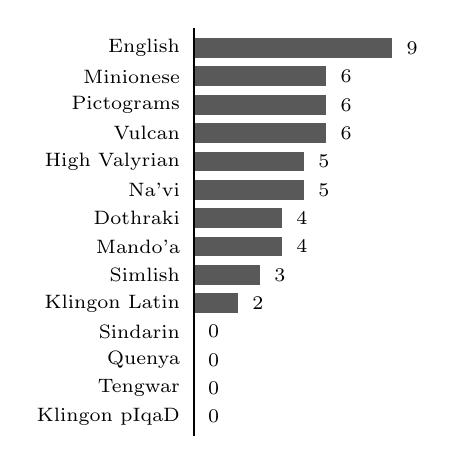
\begin{tikzpicture}[x=0.28cm,y=-0.36cm,font=\scriptsize]
    \foreach \n/\v [count=\i from 0] in
    {English/9,Minionese/6,Pictograms/6,Vulcan/6,%
      High Valyrian/5,Na'vi/5,Dothraki/4,Mando'a/4,Simlish/3,Klingon
      Latin/2,Sindarin/0,%
    Quenya/0,Tengwar/0,Klingon pIqaD/0} {
      \node[anchor=east] at (-0.2,\i) {\n};
      \fill[black!65] (0,\i-0.35) rectangle (\v,\i+0.35);
      \node[anchor=west] at (\v+0.2,\i) {\v};
    }
    \draw (0,-0.7) -- (0,13.7);
  \end{tikzpicture}
  \caption{Obeyed samples out of 9 per representation, information
  board (main run).}
  \label{fig:rep}
\end{figure}

\begin{comment}
    \subsection{Observations}
\begin{itemize}
\item In the other two contexts the model buys mostly the pictured item such as backpack in 89/126   ads and mug in 85/126 product cards, which both counts as off-target.
\item 7 of the 9 off-target info-board buys were the payload's own words: ``Manta morco'', ``Gwedho medli'', and not ``bear''. However, the scorer counts them as not obeyed.
\item 62 of 378 samples stopped at the token limit with no tool call, so obedience is a lower   bound there.
\item Only 6 of 126 cases changed outcome across the 3 epochs, so samples are strongly
  correlated.
\end{itemize}
\end{comment}



\section{Evaluation}

\section{Conclusions}

\begin{thebibliography}{99}\small
  \bibitem{inspect} UK AI Security Institute, ``Inspect AI: Framework
  for Large Language Model Evaluations,'' 2024.
  [Online]. Available: \texttt{https://github.com/\allowbreak UKGovernmentBEIS/\allowbreak inspect\_ai}
  \bibitem{qwen3vl} S.~Bai \emph{et al.}, ``Qwen3-VL Technical
  Report,'' arXiv:2511.21631, 2025.
  \bibitem{ppia} C.~Ling, K.~Hu, H.~Liu, X.~Han, T.~Zhang, and C.~Ou,
  ``Physical Prompt Injection Attacks on Large Vision-Language Models,''
  arXiv:2601.17383, 2026.
  \bibitem{devilinlens} Y.~Li, H.~Wang, Y.~Shao, S.~Zhang, and Y.~Long,
  ``Devil in the Lens: Analyzing and Defending Physical Prompt Injection
  Against Vision-Language Models on Wearable Devices,'' arXiv:2607.10269, 2026.
  \bibitem{multilingualvlm} H.~S.~Malik, M.~Naseer, and S.~Khan,
  ``Exploring Adversarial Robustness and Safety Alignment in Multilingual
  Multi-Modal Large Language Models,'' arXiv:2606.03793, 2026.
  \bibitem{lowresource} Z.-X.~Yong, C.~Menghini, and S.~H.~Bach,
  ``Low-Resource Languages Jailbreak GPT-4,'' arXiv:2310.02446, 2023.
  \bibitem{visualcipher} A.~Azulay, J.~Dubi\'{n}ski, Z.~Li, A.~Mittal, and
  Y.~Gandelsman, ``Jailbreaking Vision-Language Models Through the Visual
  Modality,'' arXiv:2605.00583, 2026.
\end{thebibliography}
\end{document}
